% (c) 2014 Daniele Masini - d.masini.it@gmail.com

\chapter{Logica di base}

\section{Proposizioni}

La logica è una scienza, e un'arte, che si occupa del modo corretto di ragionare, ossia del modo corretto di passare da certe premesse a certe conclusioni. La \emph{logica matematica} è una branca della logica, che utilizza un linguaggio simbolico e un sistema di calcolo di tipo algebrico. Questo tipo di logica, detta anche formale, fornisce uno strumento per formalizzare il linguaggio naturale.

La logica proposizionale considera come unità base dello studio le \emph{proposizioni}.

Assumiamo come primitivo, cioè senza darne una definizione, il concetto di proposizione: chiamiamo \emph{proposizione} una frase (affermativa o negativa) a cui abbia senso associare un valore di verità: vero, \emph{V}, oppure falso, \emph{F} (si usano anche i simboli 0 per falso e 1 per vero).
Per esempio, sono proposizioni logiche affermazioni del tipo:
%\begin{multicols}{2}
\begin{enumeratea}
\item <<Roma è la capitale d'Italia>>;
\item <<2+3=10>>;
\item <<5 è un numero dispari>>;
\item <<Un triangolo ha quattro angoli>>.
\end{enumeratea}
%\end{multicols}
Le frasi a) e c) sono vere mentre le frasi b) e d) sono false. Tutte quante sono pertanto delle proposizioni nel senso della logica matematica.
Non sono proposizioni logiche, invece, le frasi:
%\begin{multicols}{2}
\begin{enumeratea}
\item <<\np{1000} è un numero grande>>;
\item <<Il quadrato è una figura semplice>>;
\item <<Roma è una bella città>>;
\item <<Mi piacerebbe essere promosso>>;
\item <<Studia!>>.
\end{enumeratea}
%\end{multicols}
Queste frasi esprimono affermazioni non valutabili oggettivamente, di esse non si può dire se sono vere o false. Non sono proposizioni logiche le domande, le esclamazioni, i comandi.

Le proposizioni possono essere semplici affermazioni (\emph{proposizioni atomiche}) oppure possono essere ottenute da una o più proposizioni elementari legate tra di loro attraverso connettivi logici (elementi linguistici del tipo ``non'', ``e'', ``o'', ``se \ldots{} allora'', ``se e solo se''). In questo caso si parla di \emph{proposizioni composte} o molecolari.

Per esempio, la proposizione <<un triangolo ha tre lati e tre angoli>> è composta dalle proposizioni <<un triangolo ha tre lati>> e <<un triangolo ha tre angoli>> unite dal connettivo ``e''.

La valutazione della verità o falsità di una proposizione composta dipende dalla verità di ogni singola proposizione che la compone e da come esse sono collegate tra di loro.

\vspazio\ovalbox{\risolvi \ref{ese:6.1}}

\section{Algebra delle proposizioni}

Vediamo ora il calcolo algebrico con le proposizioni. Si usa indicare le proposizioni con lettere minuscole, tipo $p$, $q$, $r$, \ldots

La \emph{congiunzione} di due proposizioni si ottiene con il connettivo ``e'' (\emph{et}, \emph{and}, $\wedge$): la proposizione $r$ ottenuta dalla congiunzione delle proposizioni $p$ e $q$, in simboli si usa scrivere $r=p\wedge q$, è vera se entrambe le proposizioni $p$ e $q$ sono contestualmente vere, mentre è falsa quando anche una sola delle due proposizioni è falsa.

Per esempio, <<Ho avuto 7 in italiano e matematica>> è un'affermazione vera solo quando ho avuto 7 in entrambe le materie. Oppure, <<Per guidare il motorino occorre aver compiuto 14 anni e possedere il patentino>> significa che posso guidare il motorino solo se ho entrambi i requisisti: aver compiuto 14 anni e avere il patentino.

Per esprimere in maniera sintetica tutte le possibilità del valore di verità di una proposizione composta, si usa una tabella a doppia entrata, detta \emph{tavola di verità}~(tabella~\ref{tab:cong}). %, che per la congiunzione logica è la seguente

%\begin{center}
% \begin{tabular*}{.2 \textwidth}{@{\extracolsep{\fill}}*{3}{c}}
% \toprule
%$p$ &$q$ &$p\wedge q$\\
%\midrule
%V & V & V \\
%V & F & F \\
%F & V & F \\
%F & F & F \\
%\bottomrule
% \end{tabular*}
%\end{center}

La \emph{disgiunzione} (inclusiva) di due proposizioni si ottiene con il connettivo ``o'' (\emph{vel}, \emph{or}, $\vee$): la proposizione $s$ ottenuta dalla disgiunzione di due proposizioni $p$ e $q$, in simboli $s=p\vee q$, è vera quando almeno una delle due proposizioni è vera ed è falsa solo se entrambe le proposizioni sono false. % Di seguito riportiamo la relativa tavola di verità.
%\begin{center}
% \begin{tabular*}{.2 \textwidth}{@{\extracolsep{\fill}}*{3}{c}}
% \toprule
%$p$ &$q$ &$p\vee q$\\
%\midrule
%V & V & V \\
%V & F & V \\
%F & V & V \\
%F & F & F \\
%\bottomrule
% \end{tabular*}
%\end{center}

Ad esempio, la proposizione <<100 è minore di 1 o maggiore di 10>> è vera perché è vera una delle due affermazioni, precisamente 100 è maggiore di 10. Anche nell'affermazione <<L'autobus si ferma quando qualche persona deve scendere o salire>> la ``o'' è usata in senso inclusivo.

La \emph{disgiunzione esclusiva} di due proposizioni si ottiene con il connettivo (o congiunzione) ``o \ldots{} o'' (\emph{aut}, \emph{xor}, $\veebar$): la proposizione $t$ ottenuta dalla disgiunzione esclusiva di due proposizioni $p$ e $q$, in simboli $t=p \veebar q$, è vera quando soltanto una delle due proposizioni è vera ed è invece falsa quando le due proposizioni sono entrambe vere o entrambe false. % La sua tavola di verità è la seguente
%\begin{center}
% \begin{tabular*}{.2 \textwidth}{@{\extracolsep{\fill}}*{3}{c}}
% \toprule
%$p$ &$q$ &$p\veebar q$\\
%\midrule
%V & V & F \\
%V & F & V \\
%F & V & V \\
%F & F & F \\
%\bottomrule
% \end{tabular*}
%\end{center}

Per esempio, nell'affermazione <<oggi il Milan vince o pareggia>> la congiunzione ``o'' ha valore esclusivo.
%\begin{minipage}[b]{0.7\linewidth}

La \emph{negazione}, che si ottiene con il connettivo ``non'' (\emph{non}, \emph{not}, $\neg$), è un operatore che, a differenza dei precedenti, non lega più proposizioni ma agisce su un'unica proposizione (per questo si dice che è un operatore unario, in analogia all'operazione insiemistica di complementazione). La negazione di una proposizione $p$ è una proposizione che si indica con il simbolo $\neg p$ che risulta vera se $p$ è falsa, viceversa è falsa se $p$ è vera.

La doppia negazione equivale ad un'affermazione, cioè $\neg(\neg p)$ è equivalente a $p$.
%\end{minipage}
%\begin{minipage}[b]{0.3\linewidth}
%\begin{center}
% \begin{tabular*}{.2 \textwidth}{@{\extracolsep{\fill}}*{3}{c}}
% \toprule
%$p$ &$\neg p$ &$\neg(\neg p)$\\
%\midrule
%V & F & V \\
%F & V & F \\
%\bottomrule
% \end{tabular*}
%\end{center}
%\end{minipage}

% % % % % % % % % % % % % % % % % % % % % % % % % % % % % % % % %
\begin{table}[hbtp]
\caption{Tavole di verità}\label{tab:cong}
\centering%
\begin{minipage}[b]{0.22\linewidth}
\centering%
 \begin{tabular}{ccc} % {.5 \textwidth}{@{\extracolsep{\fill}}*{3}{c}}
 \toprule
$p$ &$q$ &$p\wedge q$\\
\midrule
V & V & V \\
V & F & F \\
F & V & F \\
F & F & F \\
\bottomrule
 \end{tabular}
\caption*{Congiunzione}
\end{minipage}
\begin{minipage}[b]{0.22\linewidth}
\centering%
 \begin{tabular}{ccc} % {.5 \textwidth}{@{\extracolsep{\fill}}*{3}{c}}
 \toprule
$p$ &$q$ &$p\vee q$\\
\midrule
V & V & V \\
V & F & V \\
F & V & V \\
F & F & F \\
\bottomrule
 \end{tabular}
\caption*{Disgiunzione}
\end{minipage}
\begin{minipage}[b]{0.28\linewidth}
\centering%
 \begin{tabular}{ccc} % {.5 \textwidth}{@{\extracolsep{\fill}}*{3}{c}}
 \toprule
$p$ &$q$ &$p\veebar q$\\
\midrule
V & V & F \\
V & F & V \\
F & V & V \\
F & F & F \\
\bottomrule
 \end{tabular}
\caption*{Disgiunzione esclusiva}
\end{minipage}
\begin{minipage}[b]{0.24\linewidth}
\centering%
 \begin{tabular}{ccc} % {.5 \textwidth}{@{\extracolsep{\fill}}*{3}{c}}
 \toprule
$p$ &$\neg p$ &$\neg(\neg p)$\\
\midrule
V & F & V \\
F & V & F \\
\bottomrule
 \end{tabular}
\caption*{Negazione}
\end{minipage}
\end{table}
% % % % % % % % % % % % % % % % % % % % % % % % % % % % % % % % %
\pagebreak
\begin{exrig}
\begin{esempio}
Date le seguenti proposizioni $p=\;$<<un triangolo ha tre lati>> (Vera), $q=\;$<<un triangolo ha tre vertici>> (Vera), $r=\;$<<un triangolo ha quattro angoli>> (Falsa), $s=\;$<<un triangolo ha tre dimensioni>> (Falsa), allora:
\begin{itemize*}
\item $p\wedge q$ è vera,~~$q\wedge r$ è falsa,~~$r\wedge s$ è falsa;
\item $p\vee q$ è vera,~~$q\vee r$ è vera,~~$r\vee s$ è falsa;
\item $p\veebar q$ è falsa,~~$q\veebar r$ è vera,~~$r\veebar s$ è falsa.
\end{itemize*}
\end{esempio}
\end{exrig}

È piuttosto semplice capire il meccanismo della negazione se applicata a proposizioni atomiche, spesso è meno intuitivo il valore di verità della negazione di una proposizione più complessa.
Ad esempio, la negazione di $p\wedge q$ non è $\neg p\wedge\neg q$ bensì $\neg p \vee \neg q$, mentre la negazione di $p\vee q$ è   $\neg p \wedge\neg q$.
Per esempio, <<Non è vero che Marco e Luca sono stati bocciati>> può voler dire che entrambi non sono stati bocciati o solo uno di loro non è stato bocciato.
In formule si hanno le seguenti equivalenze (\emph{leggi di De Morgan}):
\[\neg(p\wedge q)=\neg p\vee\neg q\qquad\text{e}\qquad\neg(p\vee q)=\neg p\wedge\neg q.\]
La verifica si può effettuare mediante la seguente tavola di verità. La quinta colonna è infatti l'opposto (negazione) della sesta e anche la settima è l'opposto (negazione) dell'ottava.
\begin{center}
 \begin{tabular*}{.7 \textwidth}{@{\extracolsep{\fill}}*{8}{c}}
 \toprule
$p$ &$q$ &$\neg p$ &$\neg q$ &$p \wedge q$ &$\neg p \vee \neg q$ &$p \vee q$ &$\neg p \wedge \neg q$\\
\midrule
V&	V&	F&	F&	V&	F&	V&	F\\
V&	F&	F&	V&	F&	V&	V&	F\\
F&	V&	V&	F&	F&	V&	V&	F\\
F&	F&	V&	V&	F&	V&	F&	V\\
\bottomrule
 \end{tabular*}
\end{center}

Due espressioni logiche si dicono \emph{equivalenti} se hanno gli stessi valori per la relativa colonna della tavola di verità.

Come per le operazioni aritmetiche anche per gli operatori logici è possibile analizzarne le proprietà. Ne indichiamo qualcuna a titolo di esempio:
\begin{itemize*}
\item $(p\wedge q)\wedge r = p\wedge (q\wedge r)$~~~proprietà \emph{associativa} della congiunzione;
\item $p\wedge q = q \wedge p$~~~proprietà \emph{commutativa} della congiunzione;
\item $p\wedge (q\vee r) = (p\wedge q)\vee(p\wedge r)$~~~proprietà \emph{distributiva} della congiunzione rispetto alla disgiunzione.
\end{itemize*}

Una proposizione che è sempre vera, indipendentemente dalla verità degli elementi che la compongono, è detta \emph{tautologia}. Un banale esempio di tautologia è una frase del tipo <<Quest'anno la Juve vince il campionato oppure non lo vince>>. Una proposizione che è sempre falsa, indipendentemente dalla verità dei suoi elementi, è detta \emph{contraddizione}. Un esempio banale di contraddizione è l'affermazione <<un numero è multiplo di 2 ed è dispari>>.

\begin{exrig}
\begin{esempio}
	La proposizione $p\wedge \neg p$ è una contraddizione in quanto è sempre falsa.
	La proposizione $p\vee \neg p$ è una tautologia in quanto è sempre vera.
\end{esempio}
\end{exrig}

\vspazio\ovalbox{\risolvii \ref{ese:6.2}, \ref{ese:6.3}, \ref{ese:6.4}, \ref{ese:6.5}, \ref{ese:6.6}, \ref{ese:6.7}, \ref{ese:6.8}, \ref{ese:6.9}}

\section{Predicati e quantificatori}

Una proposizione che fa riferimento a una proprietà o caratteristica di alcuni elementi di un insieme si chiama \emph{predicato} (o \emph{enunciato}). Le frasi formate da un predicato che ha alcuni argomenti incogniti si dicono \emph{enunciati aperti}.

Per esempio, $p =\;$<<$x$ è un numero intero maggiore di 10>> è un enunciato aperto.

Consideriamo ora le seguenti affermazioni:
\begin{itemize*}
\item <<Tutti gli uomini sono mortali>> si riferisce a un qualsiasi essere umano;
\item <<Tutti i multipli di 6 sono anche multipli di 2>> è vera per tutti i numeri multipli di 6;
\item <<Ogni numero negativo è minore di ogni numero positivo>>.
\end{itemize*}
I predicati precedenti non riguardano un elemento specifico ma una certa quantità di elementi. I termini ``tutti'' e ``ogni'', detti \emph{quantificatori universali}, indicano che una proprietà è vera per tutti gli elementi di un certo insieme. In logica matematica si usa il simbolo $\forall$ (che si legge ``per ogni'') per indicare il quantificatore universale.

Vediamo ora i seguenti predicati:
\begin{itemize*}
\item <<Esiste un numero che elevato al quadrato dà 16>>;
\item <<Alcuni numeri pari sono anche multipli di 3>>.
\end{itemize*}
Queste affermazioni esprimono proprietà che sono vere per almeno un elemento dell'insieme di riferimento: la prima frase è vera per i numeri $+4$ e $-4$, la seconda frase è vera per i numeri 6, 12, 18, \ldots{}

I termini ``c'è almeno'', ``alcuni'', ``esiste almeno uno'' si dicono \emph{quantificatori esistenziali} e si indicano con il simbolo $\exists$ (che si legge ``esiste'').

Bisogna prestare particolare attenzione quando si negano frasi in cui compaiono i quantificatori. Per esempio, la negazione di <<Tutti i gatti fanno le fusa>> non è <<Nessun gatto fa le fusa>> bensì <<Non tutti i gatti fanno le fusa>> che si può esprimere anche con il quantificatore esistenziale <<C'è almeno un gatto che non fa le fusa>>.
La negazione della frase <<L'anno scorso siamo stati tutti promossi>> non è <<L'anno scorso siamo stati tutti bocciati>> ma <<L'anno scorso c'è stato almeno uno di noi che non è stato promosso>>.
La negazione della proposizione $p =\;$<<Tutti i quadrati hanno due diagonali>> è la proposizione $\neg p =\;$<<Non tutti i quadrati hanno due diagonali>>. Il linguaggio comune ci potrebbe portare a considerare come negazione di $p$ la proposizione <<Nessun quadrato ha due diagonali>>, ma in realtà per avere la negazione della proposizione $p$ basta che esista almeno un quadrato che non abbia due diagonali.

\vspazio\ovalbox{\risolvii \ref{ese:6.10}, \ref{ese:6.11}}

\section{L'implicazione}

Nel linguaggio matematico sono comuni proposizioni del tipo <<Se $p$ allora $q$>>. Ad esempio <<Se un numero è multiplo di 12 allora è multiplo di 3>>. La frase precedente può essere espressa dicendo:
<<Essere multiplo di 12 implica essere multiplo di 3>>.

In logica frasi del tipo <<Se $p$ allora $q$>> vengono tradotte utilizzando l'operatore $\Rightarrow$ detto \emph{implicazione}.
La scrittura <<se $p$ allora $q$>> si traduce con la scrittura $p\Rightarrow q$, che si legge ``$p$ implica $q$''.
La proposizione $p$ è detta \emph{antecedente}, (o \emph{ipotesi}) e la proposizione $q$ è detta \emph{conseguente} (o \emph{tesi}).
Il significato logico della proposizione $p\Rightarrow q$ è <<tutte le volte che la proposizione $p$ è vera allora risulta vera anche la proposizione $q$>>. Ovvero non si dice niente sula caso in cui $p$ sia falsa.
Per esempio, l'affermazione <<Se c'è il sole andiamo al mare>> è falsa solo quando c'è il sole e non andiamo al mare; l'affermazione, infatti, non dice nulla se il sole non c'è: quindi se non c'è il sole si è liberi di andare o non andare al mare. Anche l'affermazione <<Se studi sarai promosso>> dice solo che se studi sarai promosso, non dice nulla per il caso in cui tu non studi, in questo caso infatti potrai essere ugualmente promosso.
La sua tavola di verità è la seguente:
\begin{center}
 \begin{tabular*}{.2 \textwidth}{@{\extracolsep{\fill}}*{3}{c}}
 \toprule
$p$ &$q$ &$p\Rightarrow q$\\
\midrule
V & V & V \\
V & F & F \\
F & V & V \\
F & F & V \\
\bottomrule
 \end{tabular*}
\end{center}
Uno degli errori logici più comuni è quello di pensare che da $p\Rightarrow q$si possa dedurre $\neg p\Rightarrow \neg q$.
Ad esempio dall'affermazione <<Se piove prendo l'ombrello>> qualcuno può pensare che si possa dedurre <<Se non piove non prendo l'ombrello>>. Riflettendoci, si intuisce che le due frasi non sono affatto consequenziali. Basta pensare che chi pronuncia la prima frase sta affermando soltanto che tutte le volte che piove prende naturalmente l'ombrello, ma non esclude la possibilità di prenderlo anche quando non piove (in effetti è saggio farlo se il cielo è coperto da nuvoloni neri!).

Così la frase (a) <<Se $x$ è multiplo di 12 allora è multiplo di 3>> non vuol dire (b) <<Se $x$ non è multiplo di 12 allora non è multiplo di 3>>, infatti la (a) è vera, mentre la (b) è falsa (si pensi ad esempio al numero 6 che non è multiplo di 12 ma è comunque multiplo di 3).

Ciò che ragionevolmente si può dedurre da $p\Rightarrow q$ è $\neg q\Rightarrow \neg p$.

Ad esempio da <<Se $x$ è multiplo di 12 allora è multiplo di 3>> si può dedurre <<Se $x$ non è multiplo di 3 allora non è multiplo di 12>>.

Data l'implicazione $p\Rightarrow q$ la proposizione $p$ viene detta \emph{condizione sufficiente} per $q$, mentre la proposizione $q$ viene detta \emph{condizione necessaria} per $p$.
Per esempio, studiare è condizione necessaria per essere promossi ma non è sufficiente.
Quest'ultima espressione fa appunto riferimento al fatto che da $p\Rightarrow q$ si può dedurre $\neg q\Rightarrow \neg p$. Ossia $q$ è necessaria per $p$ in quanto se non è vera $q$ non è vera neanche $p$.
Calcoliamo la tavola di verità di $p\Rightarrow q$ e di $\neg q\Rightarrow \neg p$.
\begin{center}
 \begin{tabular*}{.5 \textwidth}{@{\extracolsep{\fill}}*{6}{c}}
 \toprule
$p$ &$q$ &$p\Rightarrow q$ &$\neg q$ &$\neg p$ &$\neg q \Rightarrow \neg p$\\
\midrule
V&	V&	V&	F&	F&	V\\
V&	F&	F&	V&	F&	F\\
F&	V&	V&	F&	V&	V\\
F&	F&	V&	V&	V&	V\\
\bottomrule
 \end{tabular*}
\end{center}
Come si vede, le due proposizioni hanno gli stessi valori di verità.

In generale, data un'implicazione $p\Rightarrow q$ (\emph{proposizione diretta}):
\begin{itemize*}
\item l'implicazione $\neg p\Rightarrow \neg q$ si dice \emph{contraria} di $p\Rightarrow q$;
\item l'implicazione $q\Rightarrow p$ si dice \emph{inversa} di $p\Rightarrow q$;
\item l'implicazione $\neg q\Rightarrow \neg p$ si dice \emph{contronominale} (o \emph{controinversa}) di $p\Rightarrow q$.
\end{itemize*}

La \emph{doppia implicazione}, o \emph{equivalenza logica}, di due proposizioni $p$ e $q$ dà luogo a una proposizione che in simboli si rappresenta $p\Leftrightarrow q$ (leggasi ``$p$ se e solo se $q$'') che è vera se $p$ e $q$ sono entrambe vere o entrambe false. La tavola di verità è la seguente:
\begin{center}
 \begin{tabular*}{.65 \textwidth}{@{\extracolsep{\fill}}*{6}{c}}
 \toprule
$p$ &$q$ &$p\Leftrightarrow q$ &$p\Rightarrow q$ &$q\Rightarrow p$ &$(p \Rightarrow q) \wedge (q\Rightarrow p)$\\
\midrule
V&	V&	V&		V&	V&	V\\
V&	F&	F&		F&	V&	F\\
F&	V&	F&		V&	F&	F\\
F&	F&	V&		V&	V&	V\\
\bottomrule
 \end{tabular*}
\end{center}
L'operatore $\Leftrightarrow$ è detto di doppia implicazione perché se vale $p\Leftrightarrow q$ significa che valgono sia $p\Rightarrow q$ che $q\Rightarrow p$ (e viceversa). Nella tabella precedente, infatti, è stata messa in evidenza l'equivalenza logica tra la proposizione $p\Leftrightarrow q$ e la proposizione $(p \Rightarrow q) \wedge (q\Rightarrow p)$.

L'equivalenza logica è un relazione di equivalenza, infatti verifica le seguenti proprietà:
\begin{itemize*}
\item $p\Leftrightarrow p$\quad riflessiva;
\item se $p\Leftrightarrow q$ allora vale anche $q\Leftrightarrow p$\quad simmetrica;
\item se $p\Leftrightarrow q$ e $q\Leftrightarrow r$ allora vale anche $p\Leftrightarrow r$\quad transitiva.
\end{itemize*}

In matematica si usa spesso l'espressione <<$p$ è condizione necessaria e sufficiente per $q$>>. Per esempio <<Condizione necessaria e sufficiente affinché un numero sia divisibile per 3 è che la somma delle sue cifre sia divisibile per 3>>. Il significato della frase è che <<$p$ è sufficiente per $q$>> e inoltre <<$p$ è necessario per $q$>>. In altre parole significa dire che $p\Rightarrow q$ e $q\Rightarrow p$. Nel caso dell'esempio, <<se un numero è divisibile per 3 allora la somma delle sue cifre è divisibile per 3>>, vale quindi anche l'implicazione inversa <<se la somma delle cifre di un numero è divisibile per 3 allora il numero stesso è divisibile per 3>>.

In maniera analoga a quanto avviene per le espressioni numeriche, le espressioni logiche possono contenere varie proposizioni legate tra loro dagli operatori appena descritti ed eventualmente le parentesi che indicano la precedenza di applicazione degli operatori stessi. In linea di principio gli operatori vengono applicati nell'ordine nel quale si trovano nell'espressione da sinistra verso destra, tenendo però a mente che tra essi vige la seguente regola di precedenza: l'operatore $\neg$ ha la precedenza sugli altri, seguito dall'operatore $\wedge$ ed infine da $\vee$. Da ciò ne deriva un sistema di calcolo simbolico noto anche come algebra di Boole\footnote{matematico e logico britannico (1815 - 1864).}.

\vspazio\ovalbox{\risolvii \ref{ese:6.12}, \ref{ese:6.13}, \ref{ese:6.14}, \ref{ese:6.15}}

\subsection{I teoremi}

Un \emph{teorema} è una proposizione composta del tipo $I\Rightarrow T$, cioè una implicazione tra due proposizioni, dette \emph{ipotesi} ($I$) e \emph{tesi} ($T$). Dimostrare un teorema significa fare un ragionamento logico che permetta di concludere che la tesi è vera avendo supposto che l'ipotesi è vera.

In generale incontreremo molti teoremi che vengono denominati genericamente \emph{proposizioni}, perché il nome di ``teorema'' viene tradizionalmente attribuito solo ai teoremi più importanti. Inoltre si usa chiamare \emph{lemma} una proposizione che non ha una grande importanza di per sé, ma che è particolarmente utile per la dimostrazione di altri teoremi. Si chiama invece \emph{corollario} un teorema che è una conseguenza immediata di un altro teorema.

All'interno di una teoria matematica non è possibile dimostrare tutte le proposizioni, alcune devono essere assunte come vere senza dimostrarle, esse costituiscono la base della teoria sulle quali si fondano le dimostrazioni dei teoremi. Queste proposizioni si chiamano \emph{postulati} o \emph{assiomi}. Risulta evidente che cambiando sia pure uno solo degli assiomi cambiano anche i teoremi dimostrabili e quindi la teoria.


\subsection{La deduzione}

Nel paragrafo precedente abbiamo parlato in modo generico di implicazione, deduzione, dimostrazione. Facciamo ora un po' di chiarezza sull'uso di questi termini. L'\emph{implicazione} è un'operazione tra proposizioni, mentre la \emph{deduzione} è il ragionamento logico che costituisce la base della dimostrazione di un teorema. Per l'\emph{implicazione materiale} si usa il simbolo $\rightarrow$ mentre per la \emph{deduzione logica} si usa il simbolo $\Rightarrow$.

La frase <<Se 5 è un numero pari, allora il triangolo ha 4 lati>> è perfettamente valida da un punto di vista della logica matematica ed anzi è vera, poiché la premessa (proposizione antecedente) è falsa, per cui l'implicazione è vera anche se la proposizione conseguente è falsa (si tenga presente la tavola di verità di $p\Rightarrow q$).
Si noti però che la definizione di implicazione ha senso solamente se la premessa è vera, il suo ampliamento al caso in cui la premessa è falsa è motivata da ragioni di completezza della trattazione. Bisogna quindi fare attenzione ad usare l'implicazione logica quando la premessa è falsa. Teniamo comunque conto che se $p$ è falsa allora $(p\Rightarrow q)\wedge (p\Rightarrow \neg q)$ cioè $p\Rightarrow (q\wedge \neg q)$ è vera. Ma $q\wedge\neg q$ è una contraddizione, quindi una premessa falsa implica sempre una contraddizione.

In realtà, la dimostrazione di un teorema non è la verifica della validità dell'implicazione, anzi è un procedimento che fa uso della validità dell'implicazione stessa. In un teorema si parte dal supporre vera l'ipotesi e si dimostra, seguendo un ragionamento logico che si basa sugli assiomi e altri teoremi già dimostrati in precedenza, che anche la tesi è vera (questo se si segue il \emph{procedimento diretto}). Se si segue invece il \emph{procedimento indiretto} (o \emph{per assurdo}), si suppone che la tesi sia falsa e, sempre mediante assiomi e altri teoremi già dimostrati, si arriva, tramite passaggi logici, ad affermare che l'ipotesi è falsa (cosa che non si deve accettare).

Le principali regole del corretto ragionamento seguono alcuni schemi particolari (detti \emph{sillogismi}, dal nome ad essi attribuito da Aristotele\footnote{filosofo, scienziato e logico della grecia antica (383 o 384 \aC{} – 322 \aC).}). Presentiamo qui i quattro principali sillogismi: il \emph{modus ponens}, il \emph{modus tollens}, il \emph{sillogismo disgiuntivo} e il \emph{sillogismo ipotetico}.
\begin{center}
 \begin{tabular*}{.8 \textwidth}{@{\extracolsep{\fill}}*{6}{c}}
\toprule
 &Modus&Modus&\multicolumn{2}{c}{Sillogismo}&Sillogismo\\
 &ponens&tollens&\multicolumn{2}{c}{disgiuntivo}&ipotetico\\
\midrule
1\textsuperscript{a} premessa & $p\Rightarrow q$ & $p\Rightarrow q$ & $p\vee q$ & $p\vee q$ & $p\Rightarrow q$\\
2\textsuperscript{a} premessa & $ p $ & $ \neg q $ & $ \neg p $ & $ \neg q $  & $q\Rightarrow r$\\
\midrule
conclusione & $ q $ & $ \neg p $ & $ q $ & $ p $ & $p\Rightarrow r$\\
\bottomrule
 \end{tabular*}
\end{center}
Suggeriamo una lettura degli schemi appena esposti:
\begin{itemize}
\item \emph{modus ponens}: se sappiamo che $p$ implica $q$ e che $p$ è vera, allora possiamo concludere che anche $q$ è vera (metodo diretto di dimostrazione);
\item \emph{modus tollens}: se sappiamo che $p$ implica $q$ e che $q$ è falsa, allora possiamo concludere che anche $p$ è falsa (metodo indiretto di dimostrazione);
\item \emph{sillogismo disgiuntivo}: se sappiamo che, tra $p$ e $q$, almeno una delle due è vera, e sappiamo che $p$ (rispettivamente $q$) è falsa, allora possiamo concludere che $q$ (rispettivamente $p$) è vera;
\item \emph{sillogismo ipotetico}: se sappiamo che $p$ implica $q$ e che $q$ implica $r$, allora possiamo concludere che $p$ implica $r$ (proprietà transitiva dell'implicazione).
\end{itemize}

Altre regole (note come i \emph{giudizi} di Aristotele) fanno uso dei predicati e dei quantificatori. Riprendiamo un esempio precedente traducendo la frase <<tutti i quadrati hanno due diagonali>> e la sua negazione <<non tutti i quadrati hanno due diagonali>> in formule che fanno uso anche del linguaggio degli insiemi. Se chiamiamo $Q$ l'insieme di tutti i quadrati e $P$ la proprietà dell'avere due diagonali, se $x$ è il generico quadrato (elemento di $Q$), $P(x)$ è il predicato <<$x$ gode della proprietà $P$>>, cioè <<$x$ ha due diagonali>>, la frase <<tutti i quadrati hanno due diagonali>> si traduce in simboli: ${\forall}x\in Q$, $P(x)$.

La sua negazione è: <<esiste almeno un quadrato che non ha due diagonali>>, cioè che non gode della proprietà $P$, e si traduce in simboli così: $\exists x\in Q$, $\neg P(x)$.
In quest'ultimo caso, la virgola può anche essere sostituita da una barra verticale (``\textbar'') o da ``$:$'' e si legge ``tale che''.

Analogamente, una frase del tipo <<esiste almeno un numero naturale che sia divisore di $10$>> può scriversi come: $\exists n\in\insN\mid D(n)$, dove $D$ è la proprietà dell'essere divisore di $10$ e $D(n)$ significa che $n$ verifica la proprietà $D$, cioè che $n$ è un divisore di $10$. La sua negazione è <<nessun numero naturale è divisore di 10>>, ovvero <<preso un qualsiasi numero naturale $n$, questo non gode della proprietà $D$>>, la traduzione in simboli di tale frase è: $\forall n\in\insN$, ${\neg}D(n)$.

Mettiamo in tabella le quattro proposizioni, che corrispondono ai giudizi di Aristotele:
\begin{center}
 \begin{tabular}{cc|cc}
 \toprule
 \multirow{3}{2.5cm}{A: Giudizio universale affermativo}&$\forall x\in Q$, $P(x)$&\multirow{3}{2.5cm}{I: Giudizio particolare affermativo}&$\exists n\in\insN\mid D(n)$\\
&\multirow{2}*{$P$ è vera per ogni $x$}& &\multirow{2}*{$D$ è vera per almeno un $n$}\\
&&&\\
\midrule
 \multirow{3}{2.5cm}{E: Giudizio universale negativo}&$\forall n\in\insN$, $\neg D(n)$&\multirow{3}{2.5cm}{O: Giudizio particolare negativo}&$\exists x\in Q\mid\neg P(x)$\\
 &\multirow{2}*{$D$ è falsa per ogni $n$}& &\multirow{2}*{$P$ è falsa per almeno un $x$}\\
 &&&\\
 \bottomrule
 \end{tabular}
\end{center}

Se chiamiamo $R$ l'insieme degli elementi che verificano la proprietà $P$, e $S$ quello degli elementi che verificano la proprietà $D$, i quattro giudizi si possono rappresentare graficamente come nella figura~\ref{fig:1.1}.
\begin{figure}[b,t,h]
 \centering\begin{tikzpicture}[font=\small]
\tkzDefPoint(0,0){Y}
\tkzDefPoint(.2,0){X}
% cerchio di centro Y e raggio 1 cm
\tkzDrawCircle[R,color=blue](Y,.9 cm)
% cerchio di centro X e raggio 0.5 cm
\tkzDrawCircle[R,color=red,fill=orange!40,opacity=.5](X,.5 cm)
\node at(.2,0){X};
\node at(-.5,.4){Y};
\node at(0,1.2){A};
\node at(0,-1.3){Ogni $ x $ è $ y $};

\tkzDefPoint(2.3,0){Y}
\tkzDefPoint(4,0){X}
% cerchio di centro Y e raggio .7 cm
\tkzDrawCircle[R,color=red](Y,.7 cm)
% cerchio di centro X e raggio 0.7 cm
\tkzDrawCircle[R,color=blue](X,.7 cm)
\node at(2.3,0){X};
\node at(4,0){Y};
\node at(3.2,1.2){E};
\node at(3.2,-1.3){Nessun $ x $ è $ y $};

\tkzDefPoint(6,0){Y}
\tkzDefPoint(6.8,0){X}
% cerchio di centro Y e raggio .7 cm
\tkzDrawCircle[R,color=red](Y,.7 cm)
% cerchio di centro X e raggio 0.7 cm
\tkzDrawCircle[R,color=blue](X,.7 cm)
\node at(6.4,0){X};
\node at(7.1,.3){Y};
\node at(6.4,1.2){I};
\node at(6.4,-1.3){Qualche $ x $ è $ y $};

\begin{scope}
\tkzClipCircle[R](X,.7 cm)
\tkzDrawCircle[R,color=red,fill=orange!40,opacity=.4](Y,.7 cm)
\end{scope}

\tkzDefPoint(8.8,0){Y}
\tkzDefPoint(9.6,0){X}
% cerchio di centro Y e raggio .7 cm
\tkzDrawCircle[R,color=red,fill=orange!40,opacity=.4](Y,.7 cm)
% cerchio di centro X e raggio 0.7 cm
\tkzDrawCircle[R,color=blue](X,.7 cm)
\node at(8.5,0){X};
\node at(9.9,.3){Y};
\node at(9.2,1.2){O};
\node at(9.2,-1.3){Qualche $ x $ non è $ y $};

\begin{scope}
\tkzClipCircle[R](Y,.7 cm)
\tkzDrawCircle[R,color=red,fill=white](X,.7 cm)
\end{scope}

\end{tikzpicture}

 \caption{Rappresentazione con i diagrammi di Venn dei \emph{giudizi} di Aristotele}\label{fig:1.1}
\end{figure}


\subsection{La dimostrazione}

Tenendo conto di quanto detto precedentemente, dimostrare che $I\Rightarrow T$ significa fare un ragionamento che permetta di concludere che la tesi $T$ è vera avendo supposto che l'ipotesi $I$ sia vera.

Quando attraverso un ragionamento logico, e cioè attraverso una catena di implicazioni del tipo  $I\Rightarrow A\Rightarrow B\Rightarrow \ldots{} \Rightarrow T$, si riesce a dedurre la verità di una proposizione $T$ a partire dalla verità di una proposizione $I$, si dice che si è data una \emph{dimostrazione diretta} del teorema $I\Rightarrow T$ (attraverso le regole del modus ponens e del sillogismo ipotetico).

Un teorema può anche essere \emph{dimostrato per assurdo}, o con metodo \emph{indiretto}. Questa dimostrazione consiste nel partire dalla negazione di $T$ e, attraverso una catena di implicazioni, arrivare alla negazione di $I$ o, in generale, ad una contraddizione.

Esistono altri metodi di dimostrazione, di cui eventualmente si parlerà più diffusamente qualora si dovesse ricorrere ad essi. Per ora ci limitiamo a citarne un paio: \emph{dimostrazione per induzione} e \emph{dimostrazione mediante esempio} o \emph{controesempio}.

La \emph{dimostrazione per induzione} si usa in particolare quando vogliamo dimostrare una proprietà generale che vale per molte categorie di figure ma che non si può esprimere in maniera unica per tutte le categorie (ad esempio una proprietà che vale per tutti i poligoni ma che dipende dal numero dei lati, come l'estensione dei criteri di congruenza dei triangoli a poligoni di più lati).

Si usa invece un \emph{esempio} quando bisogna dimostrare che una certa proprietà vale per almeno un oggetto del nostro studio o un \emph{controesempio} per dimostrare che una proprietà non vale per tutti gli oggetti in esame.

Per fornire alcuni esempi di dimostrazione, avremmo bisogno di fissare prima i concetti di base e gli assiomi da cui partire, per cui rinviamo la questione al prossimo paragrafo.

Ma a cosa serve studiare la dimostrazione di un teorema? Perché non ci limitiamo ad elencare i teoremi? Per molte applicazioni basta in effetti conoscere il teorema e a volte anche soltanto la formula risolutiva. Tuttavia studiando le dimostrazioni si impara a dimostrare e quindi si impara a creare nuova matematica. Un altro importante vantaggio è che la dimostrazione spiega perché il teorema è vero e permette di scoprire la struttura nascosta nelle definizioni e nei teoremi.

Quando si studia una dimostrazione non bisogna limitarsi a leggerla e a impararla a memoria, occorre leggerla attivamente, ponendo attenzione su cosa si fa e cercando di anticipare i passaggi. Se un passaggio non è chiaro bisogna prima tornare indietro per capire come ci si è arrivati e quindi cercare di capire il motivo per cui l'autore ha messo quel passaggio. In generale, una dimostrazione va letta più volte smettendo solo quando la si è compresa a fondo.

\vspazio\ovalbox{\risolvii \ref{ese:6.16}, \ref{ese:6.17}, \ref{ese:6.18}, \ref{ese:6.19}, \ref{ese:6.20}, \ref{ese:6.21}, \ref{ese:6.22}, \ref{ese:6.23}, \ref{ese:6.24}, \ref{ese:6.25}, \ref{ese:6.26}}

\newpage

% (c) 2012 - 2014 Dimitrios Vrettos - d.vrettos@gmail.com
% (c) 2014 Claudio Carboncini - claudio.carboncini@gmail.com
\section{Esercizi}
\subsection{Esercizi dei singoli paragrafi}
\subsubsection*{\thechapter.1 - Rappresentazione tabulare}
%eliminato da Antonio
%\begin{esercizio}
%\label{ese:6.1}
%Dai una rappresentazione tabulare dell'insieme~$A$ dei numeri naturali minori di~6.
%\end{esercizio}

\begin{esercizio}
\label{ese:6.1}
Dai una rappresentazione tabulare dei seguenti insiemi
\begin{enumeratea}
 \item delle vocali della parola ``ESERCIZI'';
 \item delle lettere della parola ``RIFLETTERE'';
 \item dei numeri naturali compresi tra~6 e~12, estremi esclusi;
 \item dei numeri dispari compresi tra~10 e~20;
 \item delle lettere dell'alfabeto italiano;
 \item dei numeri naturali minori di~10;
 \item dei multipli di~7;
 \item delle preposizioni con più di due lettere;
 \item dei numeri naturali minori di~6.
\end{enumeratea}
\end{esercizio}

\begin{esercizio}
 \label{ese:6.2}
Indica in rappresentazione tabulare i seguenti insiemi.
\TabPositions{7.5cm}
\begin{enumeratea}
 \item $A=\{x\in\insN\mid x<10\}$; %\tab\dotfill
 \item $B=\{x\in\insN\mid 2\le x<5\}$; %\tab\dotfill
 \item $C=\{x\in\insN\mid 5\le x\le~10\}$; %\tab\dotfill
 \item $D=\{x\in\insN\mid 2x\le~10\}$; % \tab\dotfill
 \item $E=\{e\in\insN\mid 5\le e<10\}$; %\tab\dotfill
 \item $F=\{f\in\insN\mid f\text{ è multiplo di~3 e } f<15\}$; %\tab\dotfill
 \item $G=\{g\in\insN\mid g\text{ è una cifra del numero }121231\}$; %\tab\dotfill
 \item $H=\{h\in\insN\mid h=3n+1\text{, con }n\in\insN\}$. %\tab\dotfill
\end{enumeratea}
\end{esercizio}

\begin{esercizio}
\label{ese:6.3}
Elenca per tabulazione gli elementi di~$A=\{x\mid x\in\insN\text{, }x\text{ è pari, }x\leq10\text{, }x\neq0\}.$
\end{esercizio}

\begin{esercizio}
\label{ese:6.4}
Elenca per tabulazione gli elementi di~$L=\{l\text{ è una lettera della parola MATEMATICA}\}$.
\end{esercizio}

\subsubsection*{\thechapter.2 - Rappresentazione caratteristica}

\begin{esercizio}
\label{ese:6.5}
Descrivi mediante la proprietà caratteristica
l'insieme~$D= \{\text{S, T, U, D, I, A, R, E}\}$.
\[D=\{x\mid x\text{ è }\ldots\ldots\ldots\ldots\}\]
\end{esercizio}


\begin{esercizio}
\label{ese:6.6}
Descrivi mediante la proprietà caratteristica l'insieme
\[X=\{\text{1, 2, 3, 4, 5, 6, 7, 8, 9, 10, 11, 12, 13, 14, 15}\}.\]
\[X=\{x\in\insN\mid x\ldots\ldots\ldots\}\]
\end{esercizio}

\begin{esercizio}
\label{ese:6.7}
Descrivi mediante la proprietà caratteristica l'insieme dei numeri primi minori di~$\np{1000}$.
\end{esercizio}

\begin{esercizio}
\label{ese:6.8}
Elenca gli elementi dell'insieme~$I=\{n\in\insN\mid n\text{ è divisore di }12\}$.
\end{esercizio}

\begin{esercizio}
\label{ese:6.9}
Elenca gli elementi dell'insieme~$I=\{n\in\insN\mid n\text{ è multiplo di~3 minore di }20\}$.
\end{esercizio}
%\pagebreak
\begin{esercizio}
\label{ese:6.10}
Dato l'insieme~$A=\{\text{2, 4, 8, 16, 32, 64}\}$ quale delle seguenti proprietà caratterizzano i suoi elementi?
\begin{enumeratea}
\item $A=\{n\in\insN\mid n \text{ è numero pari minore di 65}\}$;
\item $A=\{n\in\insN\mid n\text{ è una potenza di 2}\}$;
\item $A=\{n\in\insN\mid n\text{ è una potenza di~2 minore di 65}\}$;
\item $A=\{n\in\insN\mid n=2^{m}\text{, con }m=\text{1, 2, 3, 4, 5, 6}\}$.
\end{enumeratea}
\end{esercizio}
%eliminati da Antonio e recuperati in 6.12
%\begin{esercizio}
%\label{ese:6.12}
%Indica con una proprietà caratteristica l'insieme~$B=\{\text{5, 10, 15, 20, 25, 30, 35, 40, 45, 50}\}$.
%\end{esercizio}

%\begin{esercizio}
%\label{ese:6.13}
%Indica con una proprietà caratteristica
%l'insieme~$B=\{\text{4, 9, 16, 25, 36, 49, 64, 81}\}$.
%\end{esercizio}

\begin{esercizio}
\label{ese:6.11}
Quale delle seguenti frasi indica la proprietà caratteristica
di~$A=\{\text{0, 4, 8, 12, 16, 20, }\ldots\}$
\begin{center}
\boxA\quad I multipli di~2; \quad\boxB\quad i numeri pari; \quad\boxC\quad i multipli di~4; \quad\boxD\quad i divisori di~20.
\end{center}
\end{esercizio}

\begin{esercizio}
\label{ese:6.12}
Rappresenta in forma caratteristica i seguenti insiemi.
\begin{multicols}{2}
\begin{enumeratea}
\item $A=\{\text{5, 6, 7, 8, 9, 10}\}$;
\item $B=\{\text{0, 1, 2, 3, 4, 5, \ldots, 98, 99, 100}\}$;
\item $C=\{\text{0, 3, 6, 9, 12, 15, 18, 21, 24, 27, 30}\}$;
\item $D=\{\text{5, 10, 15, 20, 25, 30, 35, 40, 45, 50}\}$;
\item $E=\{\text{4, 9, 16, 25, 36, 49, 64, 81}\}$.
\end{enumeratea}
\end{multicols}
\end{esercizio}

\begin{esercizio}
\label{ese:6.13}
Quale delle seguenti è una rappresentazione per caratteristica
dell'insieme
\[D = \{\text{0, 3, 6, 9, 12, 15, 18}\}.\]
\begin{enumeratea}
\item $D=\{x\in\insN\mid x\le~18\}$;
\item $D=\{x\in\insN\mid x\text{ è multiplo di~3 e }x<20\}$;%
\item $D=\{x\in\insN\mid x=3x\}$;
\item $D=\{x\in\insN\mid x=3\}$.
\end{enumeratea}
\end{esercizio}
%eliminato da Antonio
%\begin{esercizio}
%\label{ese:6.17}
%Rappresenta i seguenti insiemi con la proprietà caratteristica.
%\begin{enumeratea}
% \item $A=\{\text{gennaio, maggio, giugno, luglio, agosto}\}$;
% \item $B=\{\text{Gorizia, Pordenone, Trieste, Udine}\}$;
% \item $C=\{\text{sabato, domenica}\}$;
% \item $D=\{\text{10, 20, 30, 40, 50}\}$;
% \item $E=\{\text{Puglia, Piemonte}\}$.
% \end{enumeratea}
%\end{esercizio}

\begin{esercizio}
Individua una proprietà caratteristica dei seguenti insiemi numerici.
\label{ese:6.14}
\begin{enumeratea}
\spazielenx
 \item $A=\{\text{4, 9, 16, 25, \ldots}\}$;
 \item $B=\bigg\{\dfrac{1}{4}\text{, }\dfrac{1}{9}\text{, }\dfrac{1}{16}\text{, }\dfrac{1}{25}\text{, }\ldots\bigg\}$;
 \item $C=\bigg\{2\text{, }\dfrac{3}{2}\text{, }\dfrac{4}{3}\text{, }\dfrac{5}{4}\text{, }\dfrac{6}{5}\text{, }\ldots\bigg\}$;
 \item $D=\bigg\{\dfrac{1}{5}\text{, }\dfrac{1}{10}\text{, }\dfrac{1}{15}\text{, }\dfrac{1}{20}\text{, }\ldots\bigg\}$;
 \item $E=\bigg\{\dfrac{1}{4}\text{, }\dfrac{2}{9}\text{, }\dfrac{3}{16}\text{, }\dfrac{4}{25}\text{, }\dfrac{5}{36}\text{, }\ldots\bigg\}$;
 \item $F=\{+1\text{, }-2\text{, }+4\text{, }-8\text{, }+16\text{, }-32\text{, }+64\text{, }\ldots\}$.
 \end{enumeratea}
\end{esercizio}

\begin{esercizio}
\label{ese:6.15}
Rappresenta in forma caratteristica i seguenti insiemi.
\begin{enumeratea}
\item $A=\{\text{0, 2, 4, 6, 8, 10}\}$;
\item $B=\{\text{1, 4, 9, 16, 25, 36, 49, \ldots}\}$;
\item $C=\{\text{3, 4, 5, 6, 7}\}$;
\item $D=\{-5\text{, }-4\text{, }-3\text{, }-2\text{, }-1\text{, }0\text{, }+1\text{, }+2\text{, }+3\text{, }+4\text{, }+5\}$;
\item $E=\{\text{0, 10, 20, 30, 40, 50, 60, 70, 80, 90, 100}\}$;
\item $F=\{\text{1, 4, 9, 16, 25, 36, 49, 64, 81, 100}\}$.
\end{enumeratea}
\end{esercizio}

\begin{esercizio}
\label{ese:6.16}
Scrivi i primi dieci elementi dei seguenti insiemi.
\begin{enumeratea}
\spazielenx
\item $A=\{x\mid x=2n\text{, }n\in\insN\}$;
\item $B=\{x\mid x=n^{2}\text{, }n\in\insN\}$;
\item $C=\{x\mid x=2n^{2}\text{, }n\in\insN\}$;
\item $D=\{x\mid x=2n+2\text{, }n\in\insN\}$;
\item $E=\{x\mid x=n^{2}-n\text{, }n\in\insN\}$;
\item $E=\{x\mid x=\dfrac{n+1}{n-1}\text{, }x\in\insZ\text{, }n\in\insN\}$.
\end{enumeratea}
\end{esercizio}

\begin{esercizio}
\label{ese:6.17}
Elenca gli elementi dei seguenti insiemi.
\begin{multicols}{2}
\begin{enumeratea}
\item $A=\{x\in\insZ\mid -3\le x<2\}$;
\item $B=\{x\in\insN\mid -4\le x\le~1\text{ o }5<x\le~7\}$;
\item $C=\{x\in\insZ\mid -1< x\le 10\}$;
\item $D=\{x\in\insN\mid x<10\}$.
\end{enumeratea}
\end{multicols}
\end{esercizio}

\begin{esercizio}
\label{ese:6.18}
Per ciascuno dei seguenti insiemi indica alcuni elementi.
\TabPositions{6cm}
\begin{enumeratea}
\item $X=\{x\in\insN\mid x-1\text{ è pari }\}$\dotfill
\item $Y=\{y\in\insN\mid y=3n\text{, con } n\in\insN\}$\dotfill
\item $Z=\{z\in\insN\mid z=3n\text{ e } z\text{ non è divisibile per~2, }n\in\insN\}$\dotfill
\item $W=\{w\in\insN\mid w<0\}$\dotfill
\end{enumeratea}
\end{esercizio}

\subsubsection*{\thechapter.3 - Rappresentazione grafica (Diagramma di Eulero-Venn)}

\begin{esercizio}
\label{ese:6.19}
Rappresenta con un diagramma di Eulero-Venn l'insieme:
\begin{enumeratea}
\item dei multipli di~3 compresi tra~10 e~30, estremi inclusi;
\item delle note musicali;
\item dei numeri primi minori di~20;
\item delle consonanti della parola ``MATEMATICA'';
\item delle province della Toscana.
\end{enumeratea}
\end{esercizio}
%eliminato da Anronio
%\begin{esercizio}
%\label{ese:6.22}
%In base agli insiemi~$A$ e~$B$ rappresentati dai diagrammi di Eulero-Venn, stabilisci quali affermazioni sono vere.
%\begin{multicols}{2}
%\TabPositions{2.5cm}
%\begin{enumeratea}
%\item $5\notin B$\tab\boxV\quad\boxF
%\item $A=\emptyset $\tab\boxV\quad\boxF
%\item $3+2\in A$\tab\boxV\quad\boxF
%\item $B\neq \emptyset $\tab\boxV\quad\boxF
%\item $6\in B$\tab\boxV\quad\boxF
%\item $9\notin A$\tab\boxV\quad\boxF
%\end{enumeratea}
%\columnbreak
%% (c) 2012 Dimitrios Vrettos - d.vrettos@gmail.com
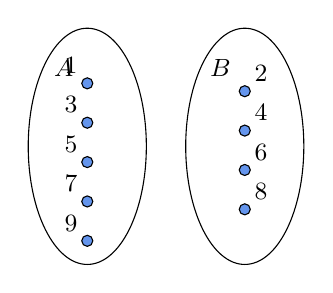
\begin{tikzpicture}[x=.5cm,y=1cm,font=\small]
    \draw (0,0)circle (1.5) (0,1) node[ left=1.5] {$A$};
    \begin{scope}[fill=CornflowerBlue, draw=black]
\filldraw (0,.8) circle (2pt) node[above left] {1};
\filldraw (0,.3) circle (2pt) node[above left] {3};
\filldraw (0,-.2) circle (2pt) node[above left] {5};
\filldraw (0,-.7) circle (2pt) node[above left] {7};
\filldraw (0,-1.2) circle (2pt) node[above left] {9};
\begin{scope}[xshift=2cm]
    \draw (0,0)circle (1.5) (0,1) node[ left=1.5] {$B$};
\filldraw (0,.7) circle (2pt) node[above right] {2};
\filldraw (0,.2) circle (2pt) node[above right] {4};
\filldraw (0,-.3) circle (2pt) node[above right] {6};
\filldraw (0,-.8) circle (2pt) node[above right] {8};
\end{scope}
\end{scope}
\end{tikzpicture}

%\end{multicols}
%\end{esercizio}

%\subsection{Esercizi riepilogativi}

\begin{esercizio}
\label{ese:6.20}
Rappresenta i seguenti insiemi con rappresentazione tabulare, caratteristica e grafica.
\begin{enumeratea}
\item Insieme~$A$ dei divisori di~30;
\item insieme~$B$ dei numeri pari minori o uguali a~10;
\item l'insieme~$C$ delle province della Puglia;
\item l'insieme~$D$ delle lettere della parola ``COCCO''.
\end{enumeratea}
\end{esercizio}

\begin{esercizio}
\label{ese:6.21}
Rappresenta nel modo che ritieni più opportuno gli insiemi i cui elementi sono:
\begin{enumeratea}
\item i numeri naturali multipli di~5 compresi tra~10 e~$\np{10000}$;
\item i colori dell'arcobaleno;
\item i numeri razionali maggiori o uguali a~$2/7$;
\item i punti di una superficie~$S$;
\item le lettere di cui è composto il tuo nome.
\end{enumeratea}
\end{esercizio}

\begin{esercizio}
\label{ese:6.22}
Rappresenta con una modalità a tua scelta l'insieme dei numeri interi multipli di~5 maggiori di~10 e minori di~100 che non
sono dispari.
\end{esercizio}
\pagebreak
\begin{esercizio}
\label{ese:6.23}
Dati gli insiemi:~$X=\{\text{8, 9, 10}\}$, $Y=\{\text{0, 8, 9, 10}\}$, $H=\{\text{10, 9, 8}\}$,
$W=\{w\in\insN\mid 8\le w\le 10\}$, $Z=\{z\in\insN\mid 8<z\le 10\}$ e~$J=\{j\in\insN\mid 7<j<11\}$,
individua le uguaglianze corrette.
\begin{multicols}{3}
\begin{enumeratea}
\item $X = Y$;
\item $X= H$;
\item $W = H$;
\item $X = Z$;
\item $\card (Z)=2$;
\item $X = J$.
\end{enumeratea}
\end{multicols}
\end{esercizio}

\begin{esercizio}
\label{ese:6.24}
Dati gli insiemi:
$A=\{$g, a, t, o$\}$, $B=\{$o, g, t, a$\}$, $C=\{c\mid c$ è una lettera della parola ``gatto''$\}$,
$D=\{$g, t$\}$, $E=\{$gatto$\}$, $F=\{f\mid f$ è una consonante della parola ``gatto''$\}$,
segna con una crocetta le uguaglianze corrette:
\begin{multicols}{4}
\begin{enumeratea}
 \item $A = B$;
 \item $A = D$;
 \item $A = C$;
 \item $E = A$;
 \item $C = E$;
 \item $D = F$;
 \item $C = D$:
 \item $D = E$.
 \columnbreak
 \item $\card (C)=5$;
 \item $\card (E)=5$;
\end{enumeratea}
\end{multicols}
\end{esercizio}
%eliminato da Antonio
%\begin{esercizio}
%Quali delle seguenti scritture sono vere?
%\begin{enumeratea}
%\TabPositions{7cm}
%\item $5\in \{\text{10, 8, 6, 4, 2}\}$\tab\boxV\quad\boxF
%\item $15\in \{n\in\insN\mid n\ge~10\}$\tab\boxV\quad\boxF
%\item $7\in \{n\in\insN\mid n+5<10\}$\tab\boxV\quad\boxF
%\item $l\notin\{x\mid x\text{ è una lettera della parola ``scuola''}\}$\tab\boxV\quad\boxF
%\end{enumeratea}
%\end{esercizio}

\begin{esercizio}
\label{ese:6.25}
Quali dei seguenti insiemi sono uguali?
 \begin{enumeratea}
 \item $A=\{1+3\text{, }5-2\text{, }1+1\text{, }9-8\text{, }1-1\}$;
\item $B=\{n\in\insN\mid n<5\}$;
\item $C=\{6-4\text{, }6+4\text{, }6-6\}$.
 \end{enumeratea}
\end{esercizio}
%\pagebreak
\begin{esercizio}
\label{ese:6.26}
Quali dei seguenti insiemi sono uguali?
\begin{multicols}{2}
\begin{enumeratea}
\item $A=\{x\in\insN\mid 3\le x\le~12\}$;
\item $B=\{x\in\insN\mid x=3\cdot n\text{, con } 1\le n\le~4\}$;
\item $A=\{x\in\insN\mid 2<x<13\}$;
\item $B=\{x\in\insN\mid x=3^{n}\text{, con }n=\text{1, 2, 3, 4}\}$.
\end{enumeratea}
\end{multicols}
\end{esercizio}


\cleardoublepage
